% Template for PLoS
% Version 3.5 March 2018
%
% % % % % % % % % % % % % % % % % % % % % %
%
% -- IMPORTANT NOTE
%
% This template contains comments intended
% to minimize problems and delays during our production
% process. Please follow the template instructions
% whenever possible.
%
% % % % % % % % % % % % % % % % % % % % % % %
%
% Once your paper is accepted for publication,
% PLEASE REMOVE ALL TRACKED CHANGES in this file
% and leave only the final text of your manuscript.
% PLOS recommends the use of latexdiff to track changes during review, as this will help to maintain a clean tex file.
% Visit https://www.ctan.org/pkg/latexdiff?lang=en for info or contact us at latex@plos.org.
%
%
% There are no restrictions on package use within the LaTeX files except that
% no packages listed in the template may be deleted.
%
% Please do not include colors or graphics in the text.
%
% The manuscript LaTeX source should be contained within a single file (do not use \input, \externaldocument, or similar commands).
%
% % % % % % % % % % % % % % % % % % % % % % %
%
% -- FIGURES AND TABLES
%
% Please include tables/figure captions directly after the paragraph where they are first cited in the text.
%
% DO NOT INCLUDE GRAPHICS IN YOUR MANUSCRIPT
% - Figures should be uploaded separately from your manuscript file.
% - Figures generated using LaTeX should be extracted and removed from the PDF before submission.
% - Figures containing multiple panels/subfigures must be combined into one image file before submission.
% For figure citations, please use "Fig" instead of "Figure".
% See http://journals.plos.org/plosone/s/figures for PLOS figure guidelines.
%
% Tables should be cell-based and may not contain:
% - spacing/line breaks within cells to alter layout or alignment
% - do not nest tabular environments (no tabular environments within tabular environments)
% - no graphics or colored text (cell background color/shading OK)
% See http://journals.plos.org/plosone/s/tables for table guidelines.
%
% For tables that exceed the width of the text column, use the adjustwidth environment as illustrated in the example table in text below.
%
% % % % % % % % % % % % % % % % % % % % % % % %
%
% -- EQUATIONS, MATH SYMBOLS, SUBSCRIPTS, AND SUPERSCRIPTS
%
% IMPORTANT
% Below are a few tips to help format your equations and other special characters according to our specifications. For more tips to help reduce the possibility of formatting errors during conversion, please see our LaTeX guidelines at http://journals.plos.org/plosone/s/latex
%
% For inline equations, please be sure to include all portions of an equation in the math environment.
%
% Do not include text that is not math in the math environment.
%
% Please add line breaks to long display equations when possible in order to fit size of the column.
%
% For inline equations, please do not include punctuation (commas, etc) within the math environment unless this is part of the equation.
%
% When adding superscript or subscripts outside of brackets/braces, please group using {}.
%
% Do not use \cal for caligraphic font.  Instead, use \mathcal{}
%
% % % % % % % % % % % % % % % % % % % % % % % %
%
% Please contact latex@plos.org with any questions.
%
% % % % % % % % % % % % % % % % % % % % % % % %

\documentclass[10pt,letterpaper]{article}
\usepackage[top=0.85in,left=2.75in,footskip=0.75in]{geometry}

% amsmath and amssymb packages, useful for mathematical formulas and symbols
\usepackage{amsmath,amssymb}

% Use adjustwidth environment to exceed column width (see example table in text)
\usepackage{changepage}

% Use Unicode characters when possible
\usepackage[utf8x]{inputenc}

% textcomp package and marvosym package for additional characters
\usepackage{textcomp,marvosym}

% cite package, to clean up citations in the main text. Do not remove.
% \usepackage{cite}

% Use nameref to cite supporting information files (see Supporting Information section for more info)
\usepackage{nameref,hyperref}

% line numbers
\usepackage[right]{lineno}

% ligatures disabled
\usepackage{microtype}
\DisableLigatures[f]{encoding = *, family = * }

% color can be used to apply background shading to table cells only
\usepackage[table]{xcolor}

% array package and thick rules for tables
\usepackage{array}

% create "+" rule type for thick vertical lines
\newcolumntype{+}{!{\vrule width 2pt}}

% create \thickcline for thick horizontal lines of variable length
\newlength\savedwidth
\newcommand\thickcline[1]{%
  \noalign{\global\savedwidth\arrayrulewidth\global\arrayrulewidth 2pt}%
  \cline{#1}%
  \noalign{\vskip\arrayrulewidth}%
  \noalign{\global\arrayrulewidth\savedwidth}%
}

% \thickhline command for thick horizontal lines that span the table
\newcommand\thickhline{\noalign{\global\savedwidth\arrayrulewidth\global\arrayrulewidth 2pt}%
\hline
\noalign{\global\arrayrulewidth\savedwidth}}


% Remove comment for double spacing
%\usepackage{setspace}
%\doublespacing

% Text layout
\raggedright
\setlength{\parindent}{0.5cm}
\textwidth 5.25in
\textheight 8.75in

% Bold the 'Figure #' in the caption and separate it from the title/caption with a period
% Captions will be left justified
\usepackage[aboveskip=1pt,labelfont=bf,labelsep=period,justification=raggedright,singlelinecheck=off]{caption}
\renewcommand{\figurename}{Fig}

% Use the PLoS provided BiBTeX style
% \bibliographystyle{plos2015}

% Remove brackets from numbering in List of References
\makeatletter
\renewcommand{\@biblabel}[1]{\quad#1.}
\makeatother



% Header and Footer with logo
\usepackage{lastpage,fancyhdr,graphicx}
\usepackage{epstopdf}
%\pagestyle{myheadings}
\pagestyle{fancy}
\fancyhf{}
%\setlength{\headheight}{27.023pt}
%\lhead{
\includegraphics[width=2.0in]{PLOS-submission.eps}}
\rfoot{\thepage/\pageref{LastPage}}
\renewcommand{\headrulewidth}{0pt}
\renewcommand{\footrule}{\hrule height 2pt \vspace{2mm}}
\fancyheadoffset[L]{2.25in}
\fancyfootoffset[L]{2.25in}
\lfoot{\today}

%% Include all macros below

\newcommand{\lorem}{{\bf LOREM}}
\newcommand{\ipsum}{{\bf IPSUM}}





\usepackage{forarray}
\usepackage{xstring}
\newcommand{\getIndex}[2]{
  \ForEach{,}{\IfEq{#1}{\thislevelitem}{\number\thislevelcount\ExitForEach}{}}{#2}
}

\setcounter{secnumdepth}{0}

\newcommand{\getAff}[1]{
  \getIndex{#1}{UC Davis,UNH}
}

\providecommand{\tightlist}{%
  \setlength{\itemsep}{0pt}\setlength{\parskip}{0pt}}

\begin{document}
\vspace*{0.2in}

% Title must be 250 characters or less.
\begin{flushleft}
{\Large
\textbf\newline{Peaks and valleys of prolatin-related gene expression during pigeon
parental care stages} % Please use "sentence case" for title and headings (capitalize only the first word in a title (or heading), the first word in a subtitle (or subheading), and any proper nouns).
}
\newline
% Insert author names, affiliations and corresponding author email (do not include titles, positions, or degrees).
\\
Rayna M Harris\textsuperscript{\getAff{UC Davis}}\textsuperscript{*},
Suzanne Austin\textsuperscript{\getAff{UC Davis}},
Andrew Lang\textsuperscript{\getAff{UNH}},
Matthew MacManes\textsuperscript{\getAff{UNH}},
Rebecca M Calisi\textsuperscript{\getAff{UC Davis}}\\
\bigskip
\textbf{\getAff{UC Davis}}UC Davis, Davis, CA\\
\textbf{\getAff{UNH}}UNH, smalltown, NH\\
\bigskip
* Corresponding author: rmharris@ucdavis\\
\end{flushleft}
% Please keep the abstract below 300 words
\section*{Abstract}
Lorem ipsum dolor sit amet, consectetur adipiscing elit.

% Please keep the Author Summary between 150 and 200 words
% Use first person. PLOS ONE authors please skip this step.
% Author Summary not valid for PLOS ONE submissions.
\section*{Author summary}
Lorem ipsum dolor sit amet, consectetur adipiscing elit.

\linenumbers

% Use "Eq" instead of "Equation" for equation citations.
\hypertarget{introduction}{%
\section{Introduction}\label{introduction}}

Understanding the mechanisms underlying parental care are critical to
circumventing issues with parent-newborn bonding as well, where ultimate
explanations are obvious, but specific mechanisms remain elusive. The
rock dove (\emph{Columba livia}) is an ideal system to characterize
changes in genetic expression during parental care transitions because:
1) ample genomic resources are available (Gillespie et al.~2013),
including a complete annotated genome assembly {[}1{]} and methodology
concerning reproductive physiology and behavior (Dong et al.~2012); and
2) rock doves are prolific, year-round breeders that thrive in
captivity, making observation, manipulation, and sampling highly
feasible year-round.

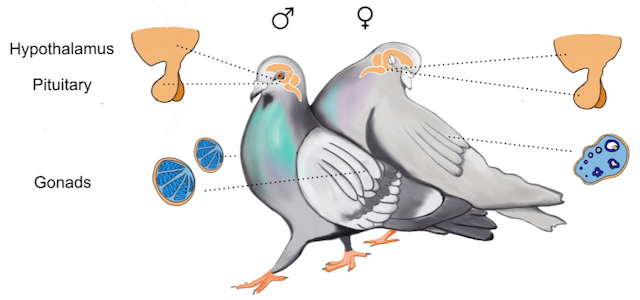
\includegraphics[width=360px]{../figures/images/PigeonHPGaxis}

Rock doves are socially monogamous and offer bi-parental care, making
inter- and intra-sexual comparisons possible. Birds offer two important
behavioral transition points into parental care: the incubation of eggs
and the caring for chicks. This produces two unique opportunities to
study how the brain transitions into two different suites of parental
care behaviors. Additionally, rock doves exhibit a parental care
strategy analogous to mammals in that they, too, `lactate' to feed their
young (Gillespie et al.~2011, 2012). This lactation, unlike simple
regurgitation of food, consists of the production and sloughing off of
skin cells inside the crop sac of females and males, creating a
protein-rich milk-like substance on which they rear their chicks. Many
functional similarities between rock dove and mammalian lactation exist
concerning the mediation of this event by the hormone prolactin (Dumont
1965). Additionally, like mammalian milk, rock dove milk delivers
essential immunoglobulins and nutritional benefits to young, aiding in
their immune function and development of microbiota {[}2{]}. Thus,
because rock doves incubate eggs and exhibit mammalian-like mediation
and function of lactation for young, they have the potential to serve as
a powerful theoretical bridge to understand the neurobiology of both
avian and mammalian transitions into parental care.

\hypertarget{materials-and-methods-and-results}{%
\section{Materials and Methods and
Results}\label{materials-and-methods-and-results}}

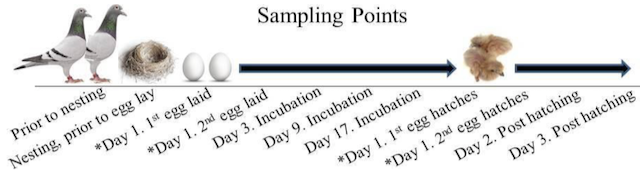
\includegraphics[width=360px]{../figures/images/samplingtimepoints}

\hypertarget{characterize-changes-in-neural-gene-expression-during-parental-care-transitions}{%
\subsection{Characterize changes in neural-gene expression during
parental care
transitions}\label{characterize-changes-in-neural-gene-expression-during-parental-care-transitions}}

Our working hypothesis is that distinct changes in transcription occur
in the brain at the anticipation of, during, and in response to two
different types of parental care: incubation behavior and hatchling
care.

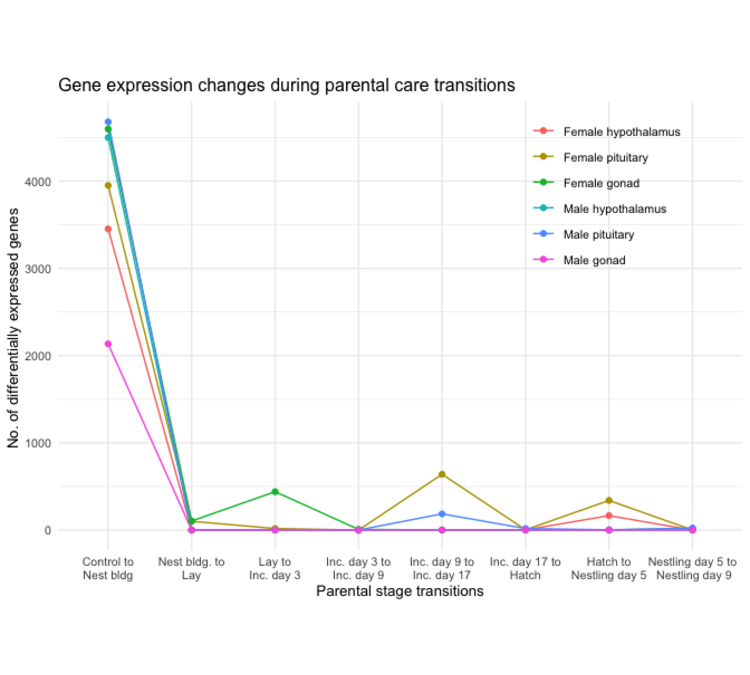
\includegraphics{characterization_manuscript_files/figure-latex/unnamed-chunk-4-1.pdf}

\textbf{Fig 2. The magnitude of gene expression changes between each
parental transition}. 4-5K genes are differentially expressed beteen
control birds and their nest buliding conspecifics in all tissues except
the male gonad. 500 - 1000 genes are differentially expressed in the
female pituitary from mid-late incubation as well as in the female
hypothalamus and pituitary from hatch to nestingly care day 5.

\hypertarget{acknowledgments}{%
\section{Acknowledgments}\label{acknowledgments}}

This project is a synergistic collaboration between the PI, Rebecca
Calisi-Rodríguez (expertise in avian behavior, parental care and
neurobiology), co-PI, Matthew MacManes (expertise in next-generation
sequencing, transcriptome assembly, and gene expression analyses), and
Collaborator, Rae Silver (expertise in neurobiology, dove behavior, and
decades of successful breeding and maintenance of dove colonies at
Barnard College).

\hypertarget{references}{%
\section*{References}\label{references}}
\addcontentsline{toc}{section}{References}

\hypertarget{refs}{}
\leavevmode\hypertarget{ref-Shapiro1063}{}%
1. Shapiro MD, Kronenberg Z, Li C, Domyan ET, Pan H, Campbell M, et al.
Genomic diversity and evolution of the head crest in the rock pigeon.
Science. American Association for the Advancement of Science; 2013;339:
1063--1067.
doi:\href{https://doi.org/10.1126/science.1230422}{10.1126/science.1230422}

\leavevmode\hypertarget{ref-Gillespie2012}{}%
2. Gillespie MJ, Stanley D, Chen H, Donald JA, Nicholas KR, Moore RJ, et
al. Functional Similarities between Pigeon `Milk' and Mammalian Milk:
Induction of Immune Gene Expression and Modification of the Microbiota.
Salmon H, editor. PLoS ONE. Public Library of Science; 2012;7: e48363.
doi:\href{https://doi.org/10.1371/journal.pone.0048363}{10.1371/journal.pone.0048363}

\nolinenumbers


\end{document}

